\documentclass{SeminarV2}
\usepackage{graphicx}
\usepackage[latin1]{inputenc}
\usepackage{amssymb,amsmath,array}

%***********************************************************************
% !!!! IMPORTANT NOTICE ON TEXT MARGINS !!!!!
%***********************************************************************
%
% Please avoid using DVI2PDF or PS2PDF converters: some undesired
% shifting/scaling may occur when using these programs
% It is strongly recommended to use the DVIPS converters.
%
% Check that you have set the paper size to A4 (and NOT to letter) in your
% dvi2ps converter, in Adobe Acrobat if you use it, and in any printer driver
% that you could use.  You also have to disable the 'scale to fit paper' option
% of your printer driver.
%
% In any case, please check carefully that the final size of the top and
% bottom margins is 5.2 cm and of the left and right margins is 4.4 cm.
% It is your responsibility to verify this important requirement.  If these margin requirements and not fulfilled at the end of your file generation process, please use the following commands to correct them.  Otherwise, please do not modify these commands.
%
\voffset 0 cm \hoffset 0 cm \addtolength{\textwidth}{0cm}
\addtolength{\textheight}{0cm}\addtolength{\leftmargin}{0cm}

%***********************************************************************
% !!!! USE OF THE SeminarV2 LaTeX STYLE FILE !!!!!
%***********************************************************************
%
% Some commands are inserted in the following .tex example file.  Therefore to
% set up your Seminar submission, please use this file and modify it to insert
% your text, rather than staring from a blank .tex file.  In this way, you will
% have the commands inserted in the right place.

% Edited by Martin Bogdan.

\begin{document}
%style file for Seminar manuscripts
\title{Was kann durch eine C++ Implementierung der DNA Histonmodifikation erreicht werden?}

%***********************************************************************
% AUTHORS INFORMATION AREA
%***********************************************************************
\author{Max Hild
% DO NOT MODIFY THE FOLLOWING '\vspace' ARGUMENT
\vspace{.3cm}\\
%
% Addresses and institutions (remove "1- " in case of a single institution)
\emph{Abgegeben bei: Dr. J{\"o}rg Galle, Prof. Dr. Markus Scholz}
% Remove the next three lines in case of a single institution
\vspace{.1cm}\\
Universit{\"a}t Leipzig, Institut f{\"u}r medizinische Informatik, Statistik und Epidemiologie\\
Neues Augusteum, Augustuspl. 10, 04109 Leipzig - Germany
}


%***********************************************************************
% END OF AUTHORS INFORMATION AREA
%***********************************************************************

\maketitle

\begin{abstract}
  \sloppy
  GWAS (Genome-Wide Association Studies) sind eine der am weitesten verbreiteten Methoden
  zur Identifizierung von genetischen Varianten, die mit komplexen Erkrankungen assoziiert sein k{\"o}nnten.
  Einer der treibenden Faktoren der Weiterentwicklung der Forschung zum menschlichen Genom
  war in den letzten Jahren jedoch eine Abkehr von der klassischen Sichtweise, dass die
  gesamte Heritabilit{\"a}t von Ph{\"a}notypen lediglich durch die genetische Kodierung
  erkl{\"a}rt werden kann. In GWAS erreichten die relevanten Ma{\ss}zahlen f{\"u}r die Heritabilit{\"a}t
  wiederholt lediglich kleine Werte. \cite{mcclellan-2010}
    
  Hier zeigte sich, dass es eine Reihe weiterer Forschungszweige wie die Transkriptionsanalyse
  sowie die Epigenetik notwendig sind, um die fehlende Heritabilit{\"a}t der Ph{\"a}notypen zu erkl{\"a}ren. 
  Epigenetische Mechanismen wie DNA-Methylierung und Histonmodifikationen spielen eine entscheidende 
  Rolle bei der Regulation der Genexpression und k{\"o}nnten somit einen Teil der "verlorenen" Heritabilit{\"a}t 
  aufkl{\"a}ren. Diese Mechanismen sind dynamisch und k{\"o}nnen durch Umweltfaktoren beeinflusst werden, 
  was sie zu einem spannenden Forschungsfeld macht.
  \end{abstract}
  

\section{Einleitung}
Die Heritabilit{\"a}t von Ph{\"a}notypen besser zu verstehen l{\"a}sst Forscherinnen und Forscher leichter
nachvollziehen, wie die genetische Information kodiert ist.
Prohaska et al. argumentieren, dass die Bedeutung des regulatorischen Systems der Epigenetik f{\"u}r die Vererbung gro{\ss} ist.
\cite{prohaska-2010}
Diese Sichtweise deckt sich mit der Ansicht von McClellan et al,
die in ihrer Arbeit die Ergebnisse der GWAS relativieren.
\begin{quote}
  \sloppy
  Eine der gr{\"o}{\ss}en Hoffnungen an die GWAS war, dass man - genauso wie eine Vielzahl von mendelschen Erkrankungen auf DNA-Ebene eingegrenzt und das beteiligte Gen samt den Mutationen identifiziert werden konnte - einfach von Einzelgen-Erkrankungen auf komplexe multigenetische Erkrankungen schlie{\ss}en k{\"o}nnte. Das ist jedoch nicht eingetreten. Bef{\"u}rworter werden argumentieren, dass es funktioniert hat und dass allerlei faszinierende Gene identifiziert wurden, die beispielsweise eine Pr{\"a}disposition zu oder einen Schutz vor Diabetes oder Brustkrebs verleihen, aber die Tatsache bleibt, dass der Gro{\ss}teil der Erblichkeit in diesen Erkrankungen nicht den durch GWAS identifizierten Loci zugeschrieben werden kann, was eindeutig zeigt, dass dies nicht die universelle L{\"o}sung sein wird.
\end{quote}
\cite{mcclellan-2010}
Zu verstehen, wie die Modifikation der Histone und DNA-Methylierung funktioniert, ist daher ein wesentlicher Schritt, um die L{\"u}cke in unserem Verst{\"a}ndnis der Heritabilit{\"a}t zu schlie{\ss}en.

\section{Methoden}
\subsection{Modellierung der Histonmodifikation}
Zur Modellierung der DNA-Histonmodifikation wurde eine C++ Implementierung entwickelt, die auf dem Modell von Prohaska et al. basiert. Das Modell simuliert die dynamischen Ver{\"a}nderungen der epigenetischen Zust{\"a}nde an CpG-Stellen {\"u}ber die Zeit. Jede CpG-Stelle kann einen von f{\"u}nf m{\"o}glichen Zust{\"a}nden annehmen:
\begin{itemize}
    \item U: Unmethyliert
    \item M: Methyliert
    \item H: Histon-modifiziert
    \item F: Vollst{\"a}ndig modifiziert (methyliert und Histon-modifiziert)
    \item C: Komplex-gebunden
\end{itemize}

Die {\"u}berg{\"a}nge zwischen diesen Zust{\"a}nden werden durch ein stochastisches Modell gesteuert, das die biologischen Prozesse der Modifikation und Demodifikation nachbildet. Die Implementierung verwendet einen Markov-Prozess, bei dem die {\"u}bergangswahrscheinlichkeiten von den aktuellen Zust{\"a}nden benachbarter CpG-Stellen abh{\"a}ngen.

\subsection{Implementierungsdetails}
Die C++ Implementierung besteht aus mehreren Klassen, die die verschiedenen Komponenten des Modells repr{\"a}sentieren:
\begin{itemize}
    \item Eine \texttt{CpGSite}-Klasse, die den Zustand einer einzelnen CpG-Stelle verwaltet
    \item Eine \texttt{Genome}-Klasse, die eine Sammlung von CpG-Stellen darstellt
    \item Eine \texttt{Simulator}-Klasse, die die zeitliche Entwicklung des Systems steuert
\end{itemize}

Die Simulation erzeugt bei jedem Zeitschritt eine neue Konfiguration aller CpG-Zust{\"a}nde basierend auf den {\"u}bergangsregeln. Die Ergebnisse werden in einer CSV-Datei gespeichert, die anschlie{\ss}end zur Visualisierung verwendet wird.

\section{Ergebnisse}
Die Simulation erm{\"o}glicht es, die zeitliche Entwicklung der epigenetischen Zust{\"a}nde {\"u}ber mehrere Generationen zu beobachten. Abbildung \ref{fig:cpg_states} zeigt die Visualisierung der Simulation.

\begin{figure}[htbp]
    \centering
    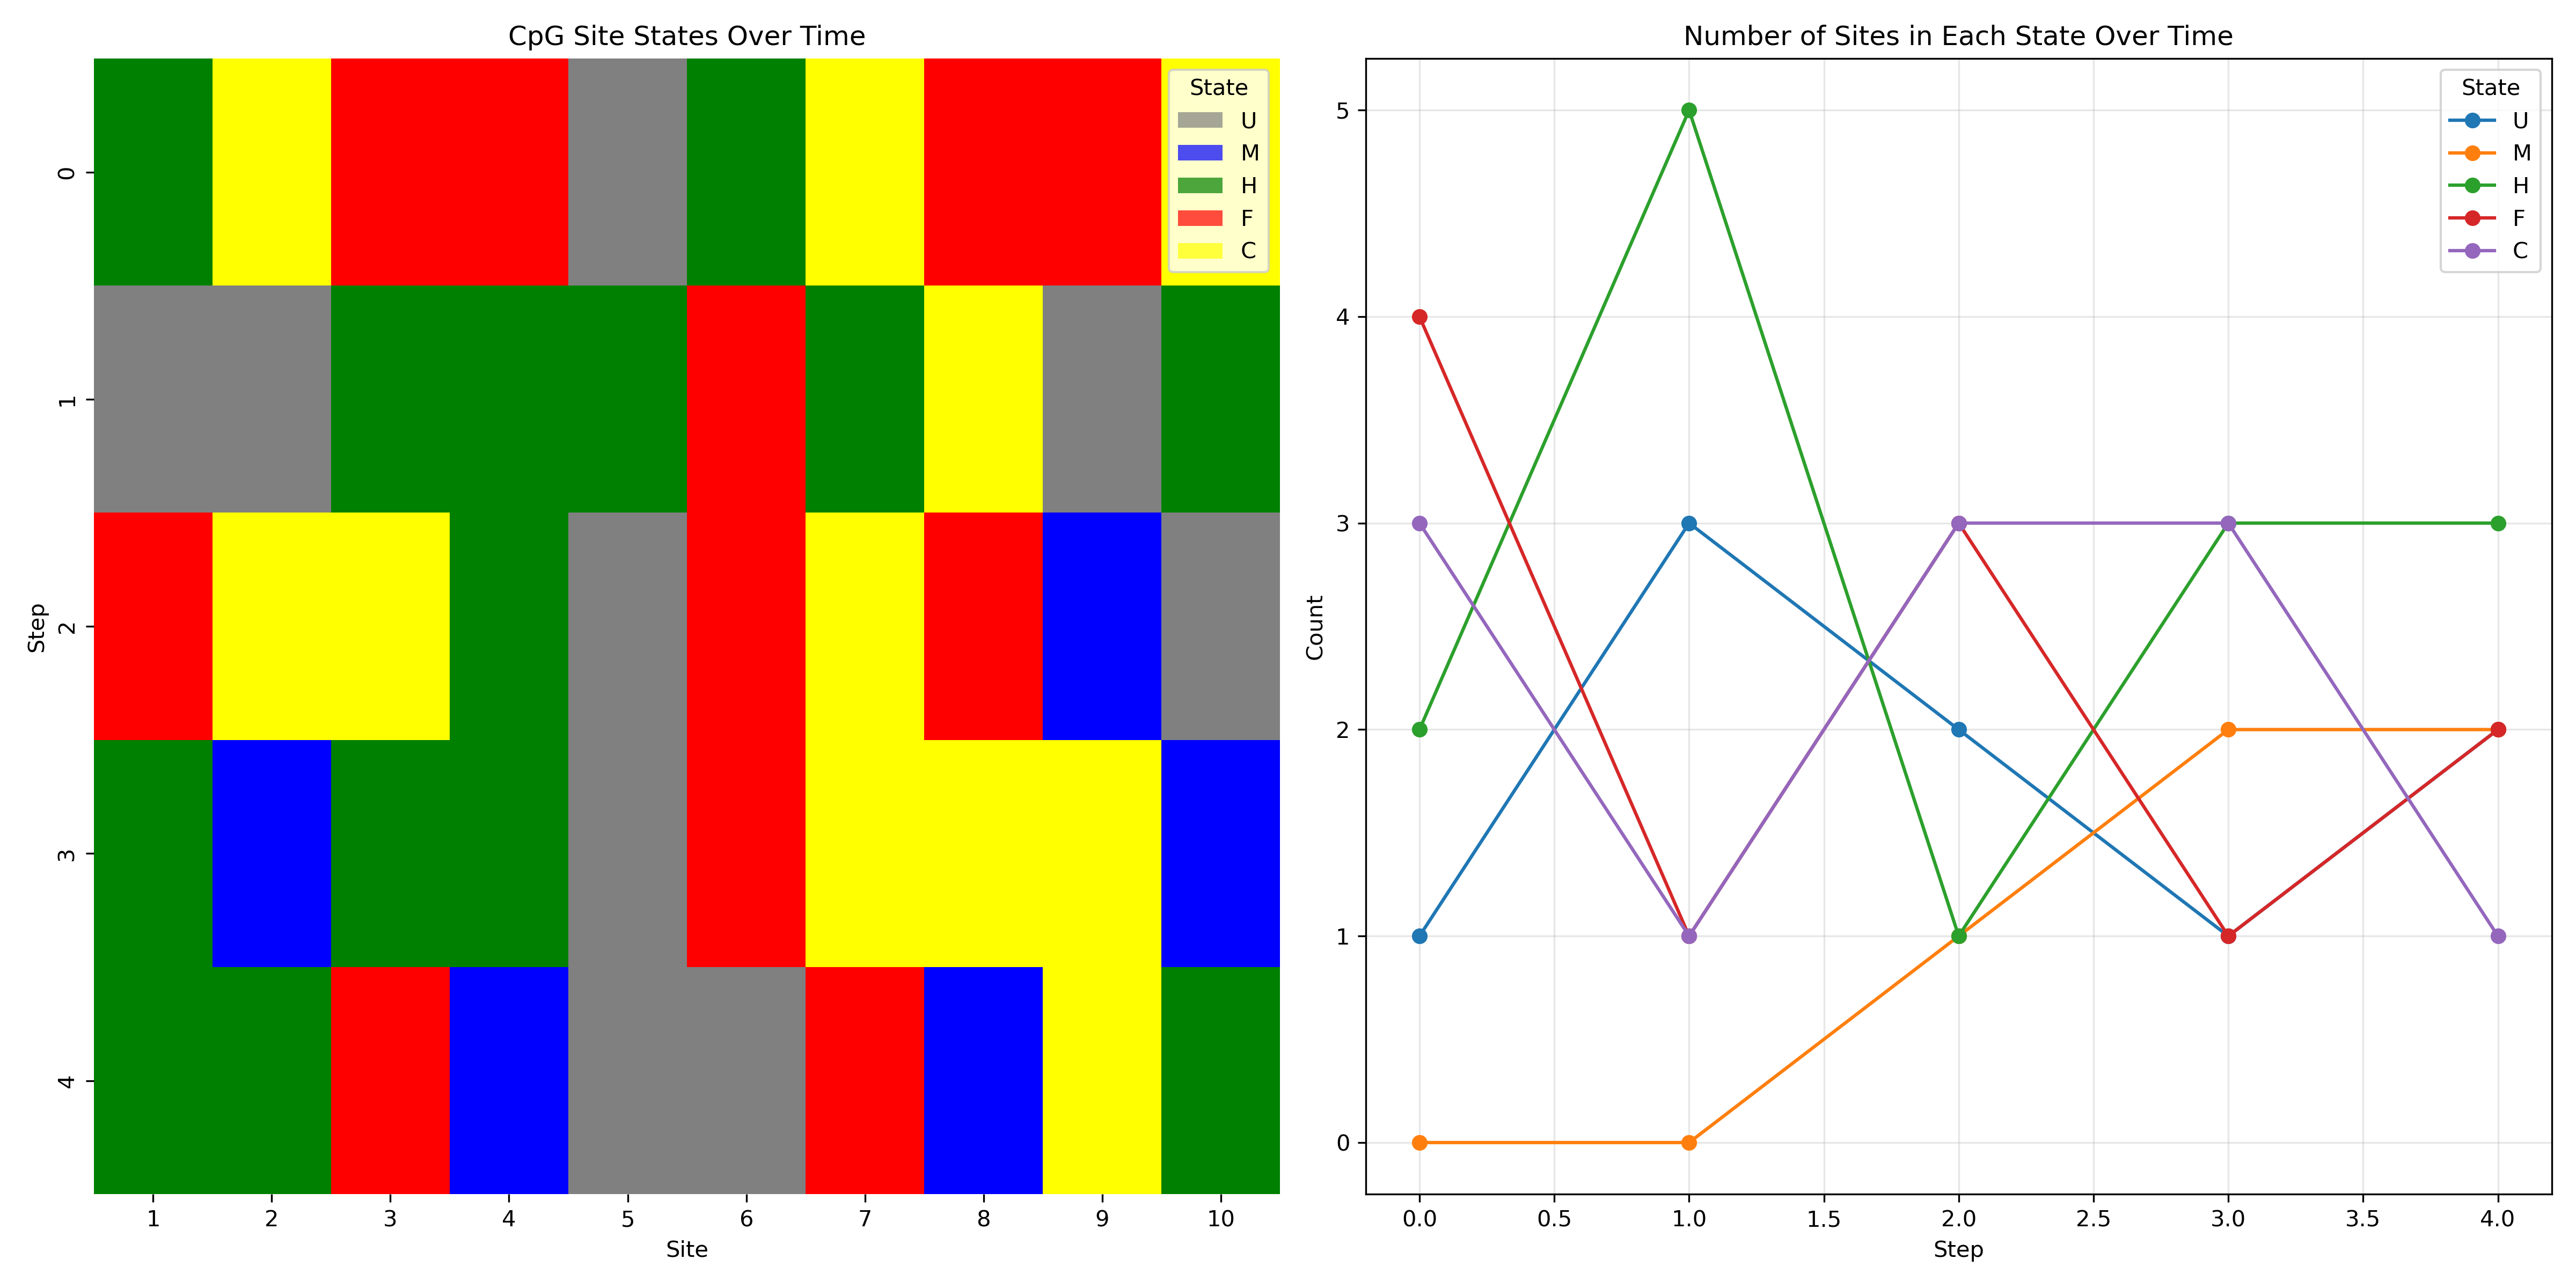
\includegraphics[width=0.9\textwidth]{cpg_states_plot.png}
    \caption{Visualisierung der CpG-Zust{\"a}nde {\"u}ber die Zeit. Links: Heatmap der Zust{\"a}nde an verschiedenen CpG-Stellen {\"u}ber die Zeit (U: grau, M: blau, H: gr{\"u}n, F: rot, C: gelb). Rechts: Anzahl der CpG-Stellen in jedem Zustand {\"u}ber die Zeit.}
    \label{fig:cpg_states}
\end{figure}

Die Visualisierung besteht aus zwei Teilen: 
\begin{enumerate}
    \item Eine Heatmap, die den Zustand jeder einzelnen CpG-Stelle {\"u}ber die Zeit darstellt
    \item Ein Liniendiagramm, das die H{\"a}ufigkeit jedes Zustands {\"u}ber die Zeit zeigt
\end{enumerate}

Die Ergebnisse zeigen deutliche Muster in der r{\"a}umlichen und zeitlichen Verteilung der epigenetischen Zust{\"a}nde. Insbesondere kann man beobachten, wie sich die Methylierungszust{\"a}nde in bestimmten Regionen zusammenh{\"a}ufen und wie sich diese Cluster {\"u}ber die Zeit entwickeln.

\section{Diskussion}
Die C++ Implementierung des Modells bietet mehrere wichtige Vorteile:

\subsection{Recheneffizienz}
Durch die Verwendung von C++ kann die Simulation effizienter durchgef{\"u}hrt werden als mit interpretierten Sprachen wie Python oder R. Dies erm{\"o}glicht die Simulation gr{\"o}{\ss}erer Genome {\"u}ber l{\"a}ngere Zeitr{\"a}ume, was f{\"u}r ein realistisches Modell der epigenetischen Prozesse unerl{\"a}sslich ist.

\subsection{Parametrisierbarkeit}
Das Modell erlaubt die einfache Anpassung verschiedener Parameter, wie z.B. die {\"u}bergangsraten zwischen den Zust{\"a}nden oder die Reichweite der Interaktionen zwischen benachbarten CpG-Stellen. Dies erm{\"o}glicht die systematische Untersuchung verschiedener biologischer Szenarien.

\subsection{Erweiterbarkeit}
Die objektorientierte Struktur der Implementierung macht es einfach, das Modell um zus{\"a}tzliche Funktionalit{\"a}ten zu erweitern, wie z.B. die Einbeziehung weiterer epigenetischer Mechanismen oder die Simulation von Umwelteinfl{\"u}ssen auf die epigenetischen Zust{\"a}nde.

\section{Fazit}
Die C++ Implementierung der DNA-Histonmodifikation erm{\"o}glicht ein tieferes Verst{\"a}ndnis der dynamischen Prozesse, die der epigenetischen Regulation zugrunde liegen. Durch die Kombination von effizienter Simulation und anschaulicher Visualisierung k{\"o}nnen komplexe epigenetische Muster erkannt und analysiert werden.

Diese Art der Modellierung kann dazu beitragen, die "verlorene" Heritabilit{\"a}t besser zu verstehen, indem sie aufzeigt, wie epigenetische Mechanismen zur Vererbung ph{\"a}notypischer Merkmale beitragen k{\"o}nnen. Die Ergebnisse unterst{\"u}tzen die These von Prohaska et al., dass das regulatorische System der Epigenetik eine wesentliche Rolle bei der Vererbung spielt, die {\"u}ber die klassische genetische Kodierung hinausgeht.

Zuk{\"u}nftige Erweiterungen der Implementierung k{\"o}nnten die Integration von experimentellen Daten zur Validierung des Modells sowie die Simulation spezifischer genetischer Erkrankungen umfassen, um potenzielle epigenetische Therapieans{\"a}tze zu identifizieren.

\begin{footnotesize}
\newpage
\bibliographystyle{unsrt}
\bibliography{own.bib}
\end{footnotesize}

\end{document}
